% Figure 4.4 Action Matrix (no fill, table-style headers; dissertation style)
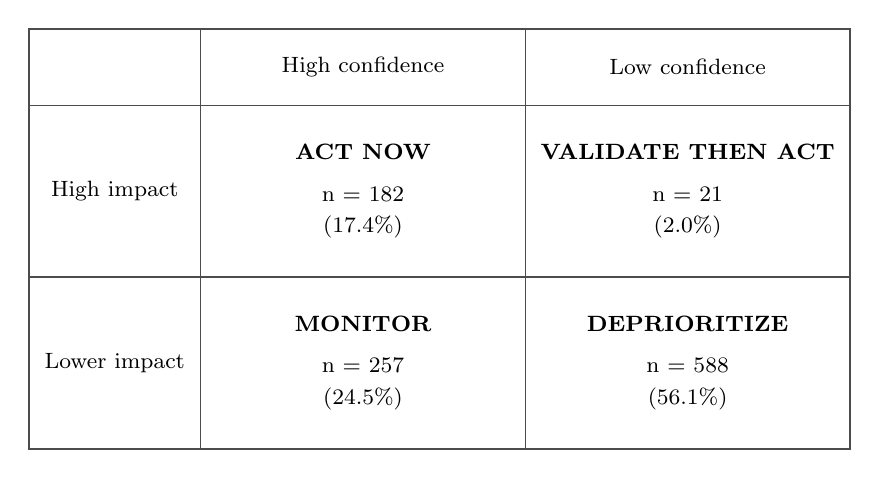
\begin{tikzpicture}

  % ---- sizing knobs ----
  \pgfmathsetlengthmacro{\AMcellw}{0.34*\linewidth}  % main cell width
  \pgfmathsetlengthmacro{\AMcellh}{0.18*\linewidth}  % main cell height
  \pgfmathsetlengthmacro{\AMhdrw}{0.18*\linewidth}   % left header column width
  \pgfmathsetlengthmacro{\AMhdrh}{0.08*\linewidth}   % top header row height

  % ---- derived geometry ----
  \pgfmathsetlengthmacro{\AMW}{\AMhdrw + 2*\AMcellw}
  \pgfmathsetlengthmacro{\AMH}{\AMhdrh + 2*\AMcellh}
  \pgfmathsetlengthmacro{\AMyMid}{\AMcellh}
  \pgfmathsetlengthmacro{\AMyTop}{2*\AMcellh}
  \pgfmathsetlengthmacro{\AMxLeft}{\AMhdrw}
  \pgfmathsetlengthmacro{\AMxMid}{\AMhdrw + \AMcellw}

  \definecolor{AMLine}{gray}{0.30}

  % ---- borders ----
  \draw[AMLine, line width=0.85pt] (0,0) rectangle (\AMW,\AMH);
  \draw[AMLine, line width=0.50pt] (\AMxLeft,0) -- (\AMxLeft,\AMH);
  \draw[AMLine, line width=0.50pt] (\AMxMid,0) -- (\AMxMid,\AMH);
  \draw[AMLine, line width=0.50pt] (0,\AMyMid) -- (\AMW,\AMyMid);
  \draw[AMLine, line width=0.50pt] (0,\AMyTop) -- (\AMW,\AMyTop);

  % ---- headers ----
  \node[align=center] at (\AMhdrw + 0.5*\AMcellw, \AMyTop + 0.5*\AMhdrh) {\footnotesize High confidence};
  \node[align=center] at (\AMhdrw + 1.5*\AMcellw, \AMyTop + 0.5*\AMhdrh) {\footnotesize Low confidence};

  \node[align=center] at (0.5*\AMhdrw, 1.5*\AMcellh) {\footnotesize High impact};
  \node[align=center] at (0.5*\AMhdrw, 0.5*\AMcellh) {\footnotesize Lower impact};

  % ---- cell text ----
  \tikzset{celltext/.style={align=center, inner sep=0pt}}

  % TOP-LEFT: ACT NOW
  \node[celltext] at (\AMhdrw + 0.5*\AMcellw, 1.5*\AMcellh) {%
    {\bfseries\footnotesize\scshape ACT NOW}\\[1.1mm]
    {\footnotesize n = 182}\\[-0.2mm]
    {\footnotesize (17.4\%)}%
  };

  % TOP-RIGHT: VALIDATE THEN ACT
  \node[celltext] at (\AMhdrw + 1.5*\AMcellw, 1.5*\AMcellh) {%
    {\bfseries\footnotesize\scshape VALIDATE THEN ACT}\\[1.1mm]
    {\footnotesize n = 21}\\[-0.2mm]
    {\footnotesize (2.0\%)}%
  };

  % BOTTOM-LEFT: MONITOR
  \node[celltext] at (\AMhdrw + 0.5*\AMcellw, 0.5*\AMcellh) {%
    {\bfseries\footnotesize\scshape MONITOR}\\[1.1mm]
    {\footnotesize n = 257}\\[-0.2mm]
    {\footnotesize (24.5\%)}%
  };

  % BOTTOM-RIGHT: DEPRIORITIZE
  \node[celltext] at (\AMhdrw + 1.5*\AMcellw, 0.5*\AMcellh) {%
    {\bfseries\footnotesize\scshape DEPRIORITIZE}\\[1.1mm]
    {\footnotesize n = 588}\\[-0.2mm]
    {\footnotesize (56.1\%)}%
  };

\end{tikzpicture}


